%%%%%%%%%%%%%%%%%%%%%%%%%%%%%%%%%%%%%%%%%
% a0poster Landscape Poster
% LaTeX Template
% Version 1.0 (22/06/13)
%
% The a0poster class was created by:
% Gerlinde Kettl and Matthias Weiser (tex@kettl.de)
% 
% This template has been downloaded from:
% http://www.LaTeXTemplates.com
%
% License:
% CC BY-NC-SA 3.0 (http://creativecommons.org/licenses/by-nc-sa/3.0/)
%
%%%%%%%%%%%%%%%%%%%%%%%%%%%%%%%%%%%%%%%%%

%----------------------------------------------------------------------------------------
%	PACKAGES AND OTHER DOCUMENT CONFIGURATIONS
%----------------------------------------------------------------------------------------

\documentclass[a0,landscape]{a0poster}

\usepackage{multicol} % This is so we can have multiple columns of text side-by-side
\columnsep=100pt % This is the amount of white space between the columns in the poster
\columnseprule=3pt % This is the thickness of the black line between the columns in the poster

\usepackage[svgnames]{xcolor} % Specify colors by their 'svgnames', for a full list of all colors available see here: http://www.latextemplates.com/svgnames-colors

\usepackage{times} % Use the times font
%\usepackage{palatino} % Uncomment to use the Palatino font

\usepackage{graphicx} % Required for including images
\graphicspath{{../Analyse/out/}} % Location of the graphics files
\usepackage{booktabs} % Top and bottom rules for table
\usepackage[font=small,labelfont=bf]{caption} % Required for specifying captions to tables and figures
\usepackage{amsfonts, amsmath, amsthm, amssymb} % For math fonts, symbols and environments
\usepackage{wrapfig} % Allows wrapping text around tables and figures
\usepackage{natbib}
\usepackage{fontawesome} % phone symbol etc.
\usepackage{arydshln} % dashed lines in table
\usepackage{enumerate}

% sans serif font
\renewcommand{\familydefault}{\sfdefault}

\renewcommand\bibsection{\subsubsection*{References}}

\begin{document}

%----------------------------------------------------------------------------------------
%	POSTER HEADER 
%----------------------------------------------------------------------------------------

% The header is divided into three boxes:
% The first is 55% wide and houses the title, subtitle, names and university/organization
% The second is 25% wide and houses contact information
% The third is 19% wide and houses a logo for your university/organization or a photo of you
% The widths of these boxes can be easily edited to accommodate your content as you see fit

\begin{minipage}[b]{0.51\linewidth}
\veryHuge \color{NavyBlue} \textbf{Let's Talk Politics} \color{Black}\\[.5cm] % Title
\Huge A Naive Approach for Measuring Political Sophistication\\[1cm] % Subtitle
\huge \textbf{Patrick W. Kraft} % Author(s)
\end{minipage}
%
\begin{minipage}[b]{0.25\linewidth}
\color{DarkSlateGray}\Large \textbf{University of Wisconsin-Milwaukee}\\
Department of Political Science\\ % Address
%\faPhone\hspace{.2em} +1 (631) 371-1607\\ % Phone number
\faEnvelope\hspace{.2em} \texttt{kraftp@uwm.edu}\\ % Email address
\faTwitter\hspace{.2em} \texttt{@patrickwkraft}\\ % Twitter
\faGlobe\hspace{.2em} \texttt{pwkraft.github.io} % Website
\end{minipage}
%
\begin{minipage}[b]{0.25\linewidth}
\includegraphics[width=.9\textwidth]{/home/patrick/Dropbox/Uni/Misc/Logos/UWM/UWM_preferred.png}
\end{minipage}
%
%\begin{minipage}[b]{0.07\linewidth}
%\color{DarkSlateGray}\Large Get Paper:\\
%
\includegraphics[width=.4\linewidth]{qr_pdf.png}
%\end{minipage}


\vspace{1cm} % A bit of extra whitespace between the header and poster content

%----------------------------------------------------------------------------------------

\begin{multicols}{4} % This is how many columns your poster will be broken into, a poster with many figures may benefit from less columns whereas a text-heavy poster benefits from more

\color{Navy} % Navy color for the abstract
\begin{abstract}
This paper proposes a simple but powerful framework to measure political sophistication based on open-ended survey responses. \textit{Discursive sophistication} utilizes automated text analysis methods to capture the complexity of individual attitude expression. I validate the approach by comparing it to conventional political knowledge metrics in multiple studies using different batteries of open-ended items. The paper then illustrates how the measure can help refine previous insights from the literature such as the oft-cited gender gap in political knowledge. Women might know fewer facts about institutions and elites, but they do not differ substantively in the sophistication of their expressed political beliefs.
\end{abstract}

\color{SaddleBrown} % SaddleBrown color for the introduction
%\color{Black}
\section*{Factual knowledge scores are problematic because they...}
\begin{enumerate}[...]
   \item ignore partial knowledge \citep[e.g.][]{debell2013harder}
   \item are biased due to guessing \citep[e.g.][]{mondak2004knowledge}
   \item convolute different types of knowledge \citep{barabas2014question}
   \item do not capture belief systems \citep{luskin1987measuring,tetlock1983cognitive}
   \item are not related to political competence \citep{lupia2006elitism}
\end{enumerate}


%\color{DarkSlateGray} % DarkSlateGray color for the rest of the content
\color{Black} % DarkSlateGray color for the rest of the content
\section*{Discursive sophistication captures the complexity in open-ended responses}
Facing a set of questions on various political issues, sophisticated respondents should be able to express a larger number of considerations, use words that are highly descriptive of each topic, and be able to voice their opinion on each issue.
\begin{align*}
\text{considerations}_i &= \dfrac{|\mathcal{T}^*_i|}{\max_i|\mathcal{T}^*_i|}\\
\text{word choice}_i &= \dfrac{\sum_{\mathcal{W}_i} P(w|t^*)}{\max_i\left[\sum_{\mathcal{W}_i} P(w|t^*)\right]}\\
\text{opinionation}_i &= \dfrac{-\sum_{j=1}^J p_{ij} \ln p_{ij}}{\ln J}\\\\
\text{sophistication}_i &= \tfrac{1}{3}(\text{considerations}_i + \text{word choice}_i + \text{opinionation}_i)
\end{align*}
\begin{center}\footnotesize
\begin{tabular}{lp{22cm}}
\toprule 
$i$ & Individual respondent \\
$\mathcal{T}^*_i$ & Set of topics mentioned by respondent $i$ (via STM, see \citealt{roberts2014structural}) \\
$\mathcal{W}_i$ & Complete set of words contained in all responses of person $i$\\
$w\in\mathcal{W}_i$ & Individual word in a response, each assigned to a topic $t^* \in \{1,...,T\} $ \\
$p_{ij}$ & Proportion of words in person $i$'s response to question $j\in \{1,...,J\}$ relative to the overall response length across all questions. \\
\bottomrule
\end{tabular}
\end{center}


\section*{Consider the following illustrative example}
\begin{center}\footnotesize
\begin{tabular}{l|p{11cm}|p{9cm}}
\toprule
	& Low Sophistication Response & High Sophistication Response \\ \midrule
Clinton (+)		& 																& Politician. \\\hdashline
Clinton (-)		& The fact that she has links to Al-Qaeda. 						& Caught in lies. \\\hdashline
Trump (+)		& 																& Says what he thinks. \\\hdashline
Trump (-)		& He is going to start a civil war. I feel like he is racist. 	& Reality TV star, poor businessman \\\hdashline
Democrats (+)	& 																& Middle class minded. \\\hdashline
Democrats (-)	& 																& Too many handouts. \\\hdashline
Republicans (+)	& 																& Economic growth conscious. \\\hdashline
Republicans (-)	& 																& For the big business. \\\midrule
Disc. Soph. 	& 0.162 														& 0.461 \\\bottomrule
\end{tabular}
\captionof{table}{\color{Green} Example of open-ended responses for low and high scores on discursive sophistication with equal factual knowledge scores (3 out of 4 correct responses) in the 2016 ANES. %Column A displays the verbatim responses of an individual who scored low on discursive sophistication and column B displays the verbatim responses of an individual who scored high on the open-ended measure. Each row represents one of the likes/dislikes items included in the analysis. Note that the responses in this table were slightly redacted for readability (spelling errors removed, etc.).
}
\end{center}


\section*{Discursive sophistication is correlated with conventional knowledge measures...}
\begin{center}\footnotesize
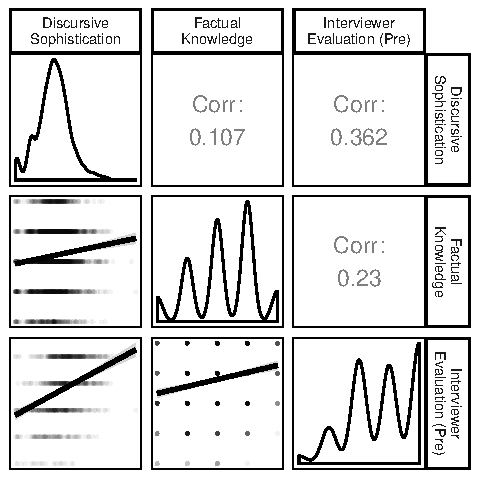
\includegraphics[width=\linewidth]{../fig/anes2016_corplot.pdf}
\captionof{figure}{\color{Green} Correlation matrix of discursive sophistication and conventional political knowledge metrics. The plots on the diagonal display univariate densities for each variable. The panels in the lower triangular display the scatter plot of two measures as well as a linear fit. The upper triangular displays the correlation coefficient. All correlations are statistically significant with $p<.05$.}
\end{center}


\section*{...but it is a better predictor of engagement and participation in politics...}
\begin{center}
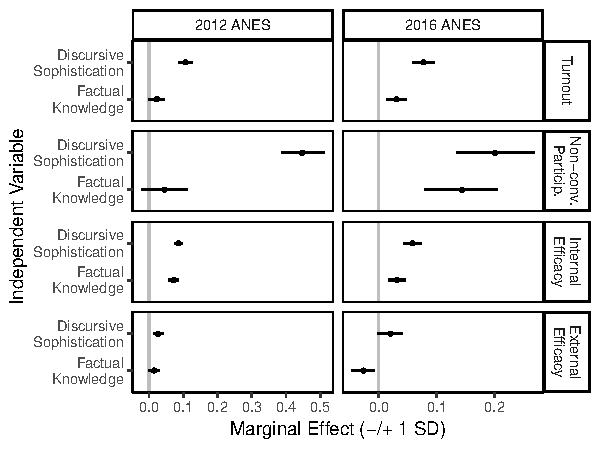
\includegraphics[width=\linewidth]{../fig/knoweff_pres_poster.pdf}
\captionof{figure}{\color{Green} Effects of sophistication on turnout, non-conventional participation, internal efficacy, and external efficacy in the 2012 and 2016 ANES. For each dependent variable, the figure displays the change in expected values after increasing each sophistication measure from -1 to +1 standard deviation from its mean (including 95\% confidence intervals). Model estimates are based on logistic regression (turnout) or OLS (non-conventional participation, internal efficacy, external efficacy). Both sophistication measures are included simultaneously while controlling for gender, education, income, age, race, church attendance, survey mode, and Wordsum vocabulary scores.}
\end{center}


\section*{...and it is positively related to manual coding of well-justified preferences}
%\subsection*{(across three languages!)}
\begin{center}
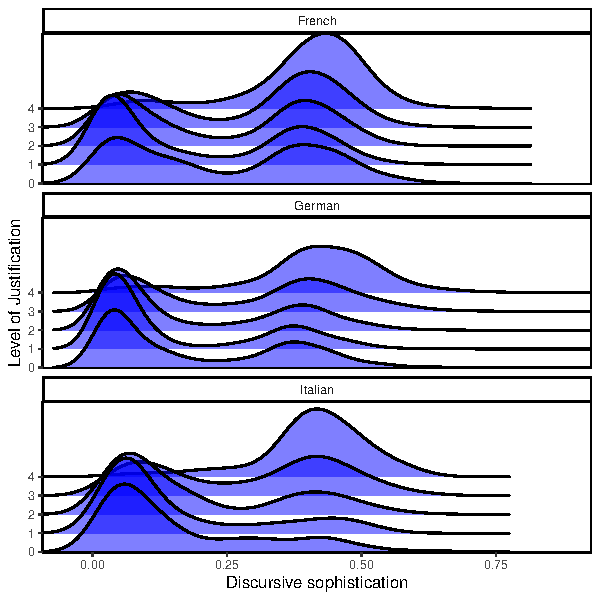
\includegraphics[width=\linewidth]{../fig/swiss_ggridges_poster.pdf}
\captionof{figure}{\color{Green} Discursive sophistication and manually coded level of justification \citep{colombo2016justifications} in Swiss post-referendum surveys. The plot compares kernel densities of discursive sophistication for each manually coded level of justification.}
\end{center}


\section*{Application: No evidence for a gender gap in discursive sophistication}
\begin{center}
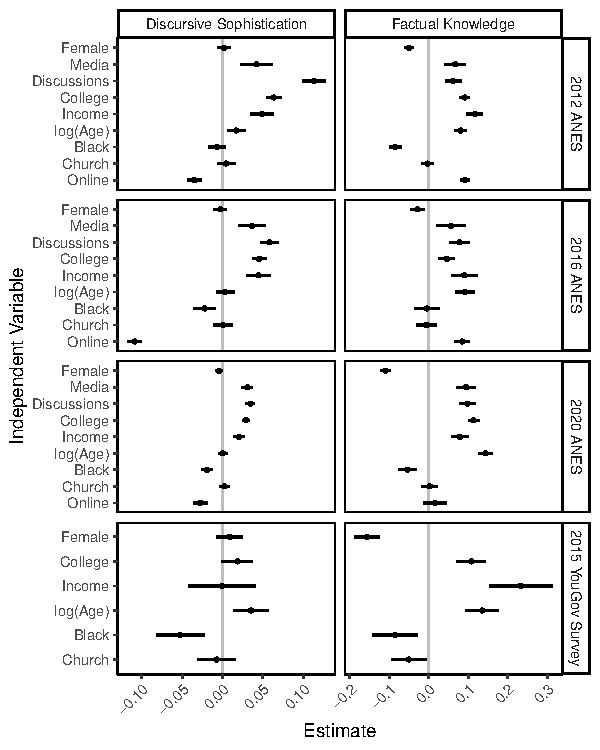
\includegraphics[width=\linewidth]{../fig/determinants_poster.pdf}
\captionof{figure}{\color{Green} Common determinants of political sophistication. Estimates are OLS regression coefficients with 95\% confidence intervals. Dependent variables are discursive sophistication as well as factual political knowledge.}
\end{center}


\section*{Why no gender gap? Women can focus on different issues in open-ended responses}
\begin{center}
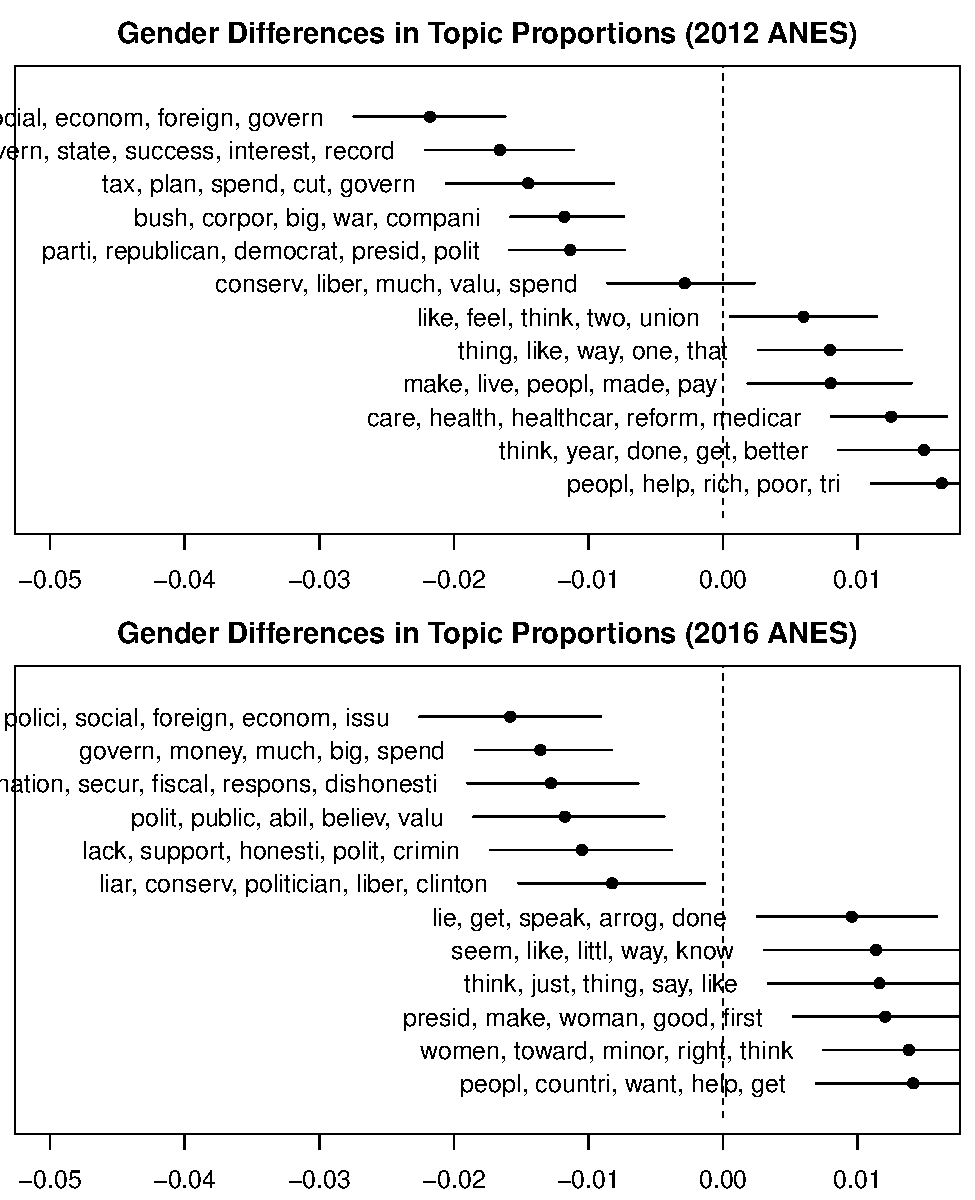
\includegraphics[width=\linewidth]{../fig/stm_gender_poster.pdf}
\captionof{figure}{\color{Green} Gender differences in topic proportions in open-ended responses based on the structural topic model used to compute discursive sophistication (including 95\% confidence intervals). Coefficients indicate the difference in predicted topic prevalence among men and women; positive values indicate higher prevalence among women. Labels are based on the five highest probability terms related to the topic.}
\end{center}


\section*{Would you like to know more?\\Download the paper here:}
\begin{center}

\includegraphics[width=.4\linewidth]{qr_pdf.png}
\end{center}

%\color{SaddleBrown} % SaddleBrown color for the introduction
%\section*{Conclusion}

%----------------------------------------------------------------------------------------

%----------------------------------------------------------------------------------------
%	REFERENCES
%----------------------------------------------------------------------------------------


\color{Black} % SaddleBrown color for the introduction
\begin{tiny}
\setlength{\parskip}{-5pt}
\bibliographystyle{/data/Dropbox/Uni/Lit/apsr2006}
\bibliography{/data/Dropbox/Uni/Lit/Literature}
\end{tiny}

%----------------------------------------------------------------------------------------
%	ACKNOWLEDGEMENTS
%----------------------------------------------------------------------------------------

%\subsubsection*{Acknowledgements}
%\setlength{\parskip}{-20pt}
%%\begin{footnotesize} 
%I thank Laura Buchanan for her work on previous versions of this paper as well as Jennifer Jerit, Yanna Krupnikov, and Stanley Feldman for helpful comments.
%%\end{footnotesize} 

%----------------------------------------------------------------------------------------

\end{multicols}
\end{document}